% Author: Izaak Neutelings (May 2021)
% Description: hadronic top quark jet
\documentclass[border=3pt,tikz]{standalone}
\usepackage{amsmath}
\usepackage{physics}
\usepackage{xcolor}
\usetikzlibrary{calc}
\usetikzlibrary{math} % for \tikzmath
\tikzset{>=latex} % for LaTeX arrow head
\colorlet{myblue}{blue!60!black}
\colorlet{mydarkblue}{blue!5!black}
\colorlet{mylightblue}{blue!60!black!5}

\begin{document}


% RESOLVED TOP JETS
\begin{tikzpicture}
  \def\N{40}
  \def\oang{26} % opening angle triangle
  \foreach\i [evaluate={\x=1.2*\i; \ang=\i*360/\N}] in {0,...,\N}{
    
    % SQUARE
    \draw[thick,mydarkblue,
      top color=mylightblue,bottom color=mydarkblue,shading angle=\ang]
        (\x,0) rectangle++ (1,1);
    \begin{scope}
      \clip (\x,0) rectangle++ (1,1);
      \draw[thick,myblue]
        (\x+0.5,0.5)++(\ang+180:1) --++ (\ang:2);
      \draw[thin,myblue,shift={(\ang-90:0.35)}]
        (\x+0.5,0.5)++(\ang+180:1) --++ (\ang:2);
      \draw[thin,myblue,shift={(\ang+90:0.35)}]
        (\x+0.5,0.5)++(\ang+180:1) --++ (\ang:2);
    \end{scope}
    
    % CIRCLE
    \draw[thick,mydarkblue,
      top color=mylightblue,bottom color=mydarkblue,shading angle=\ang]
        (\x+0.5,1.6) circle(0.5);
    \begin{scope}
      \clip (\x+0.5,1.6) circle(0.5);
      \draw[thick,myblue]
        (\x+0.5,1.6)++(\ang+180:1) --++ (\ang:2);
      \draw[thin,myblue,shift={(\ang-90:0.35)}]
        (\x+0.5,1.6)++(\ang+180:1) --++ (\ang:2);
      \draw[thin,myblue,shift={(\ang+90:0.35)}]
        (\x+0.5,1.6)++(\ang+180:1) --++ (\ang:2);
    \end{scope}
    
    % TRIANGLE
    \draw[thick,mydarkblue,
      top color=mylightblue,bottom color=mydarkblue,shading angle=\ang] %-\oang
        (\x+0.5,2.8)++(\ang-180:0.5) --++ (\ang-\oang:1) --++ (\ang+90:{2*sin(\oang)}) -- cycle;
    \begin{scope}
      \clip (\x+0.5,2.8)++(\ang-180:0.5) --++ (\ang-\oang:1) --++ (\ang+90:{2*sin(\oang)}) -- cycle;
      \draw[thick,myblue]
        (\x+0.5,2.8)++(\ang+180:1) --++ (\ang:2);
      \draw[thin,myblue,shift={(\ang-90:0.2)}]
        (\x+0.5,2.8)++(\ang+180:1) --++ (\ang:2);
      \draw[thin,myblue,shift={(\ang+90:0.2)}]
        (\x+0.5,2.8)++(\ang+180:1) --++ (\ang:2);
    \end{scope}
    
  }
\end{tikzpicture}


\end{document}